\documentclass[
    xetex,
    a4paper,
    10pt
]{scrartcl}                            %% KOMA-Script Dokumentklasse "scrartcl" verwenden

% einbinden der Pakete
\usepackage{graphicx}                          % Paket um Grafiken einbetten zu können
\usepackage[a4paper,left=0mm, bottom=0mm, top=10mm, right=0mm]{geometry} % Paket zum Einstellen der Seitenränder
\usepackage{verbatim}                        % Kommentare länger als eine Zeile (begin/end comment)
\usepackage{tikz}
    \usetikzlibrary{decorations.pathmorphing,shapes,shapes.symbols}
    \tikzstyle{border box}=[draw, very thick, decorate, decoration={random steps, segment length=3pt, amplitude=1pt}, fill=white]
    \tikzstyle{shade box}=[fill=gray!20, draw opacity=0, decorate, decoration={random steps, segment length=3pt, amplitude=1pt}]
    \tikzstyle{input box}=[fill=gray!20, rounded corners=.1cm, minimum height=5mm]
    \tikzstyle{name box}=[draw, very thick, tape, tape bend top=out and in, tape bend bottom=out and in, tape bend height=4mm, fill=white]
    \tikzstyle{level box}=[draw, very thick, fill=white, signal, signal from = east, signal to = nowhere]
    \tikzstyle{circle box}=[draw, shape=ellipse, very thick, fill=white]

\usepackage{units}

\usepackage{fontspec}
    \setmainfont{Z003}

% Setzen globaler Parameter
\graphicspath{{img/}}                     % legt globalen Pfad für Bilddateien fest
%\setlength{\parindent}{0pt}                 % unterdrückt den Absatzeinzug
%\setlength{\parskip}{0pt}         % Erstellt keine leere Zeile für jeden neuen Paragraphen

% Name and Basic Information
\newcommand{\vName}{Mwanajeshi wa mganga}
\newcommand{\vClass}{Cleric (Life Domain)}
\newcommand{\vLvl}{3}
\newcommand{\vRace}{Warforged (Envoy)}
\newcommand{\vBackground}{Acolyte}
\newcommand{\vAlignment}{chaotic good}
\newcommand{\vPlayer}{Timo}
\newcommand{\vXP}{1034}
\newcommand{\vnXP}{2700}

% Basic Stats
\newcommand{\vStr}{14}
\newcommand{\vStrMod}{+2}
\newcommand{\vDex}{11}
\newcommand{\vDexMod}{+0}
\newcommand{\vCon}{16}
\newcommand{\vConMod}{+3}
\newcommand{\vInt}{13}
\newcommand{\vIntMod}{+1}
\newcommand{\vWis}{14}
\newcommand{\vWisMod}{+2}
\newcommand{\vCha}{10}
\newcommand{\vChaMod}{+0}
\newcommand{\vSan}{10}
\newcommand{\vSanMod}{+0}

\newcommand{\vProf}{+2}
\newcommand{\vAbilitySave}{12}
\newcommand{\vPerception}{12}
\newcommand{\vInspiration}{00}

% Fight Stats
\newcommand{\vAC}{18}
\newcommand{\vtempAC}{00}
\newcommand{\vInitiative}{+0}
\newcommand{\vmaxHP}{24}

\newcommand{\vSpeed}{9.5}
\newcommand{\vHDa}{1d8}
\newcommand{\vHDaTot}{3}

% Saving throws
\newcommand{\vStrSave}{+2}
\newcommand{\vDexSave}{+0}
\newcommand{\vConSave}{+3}
\newcommand{\vIntSave}{+1}
\newcommand{\vWisSave}{+4}
\newcommand{\vChaSave}{+2}
\newcommand{\vSanSave}{+0}

\newcommand{\vStrSaveC}{white}
\newcommand{\vDexSaveC}{white}
\newcommand{\vConSaveC}{white}
\newcommand{\vIntSaveC}{white}
\newcommand{\vWisSaveC}{black}
\newcommand{\vChaSaveC}{black}
\newcommand{\vSanSaveC}{white}

% Skill checks
\newcommand{\vAcro}{+0}
\newcommand{\vAnim}{+2}
\newcommand{\vArca}{+1}
\newcommand{\vAthl}{+2}
\newcommand{\vDece}{+0}
\newcommand{\vHist}{+3}
\newcommand{\vInsi}{+4}
\newcommand{\vInti}{+0}
\newcommand{\vInve}{+1}
\newcommand{\vMedi}{+4}
\newcommand{\vNatu}{+1}
\newcommand{\vPerc}{+2}
\newcommand{\vPerf}{+0}
\newcommand{\vPers}{+2}
\newcommand{\vReli}{+3}
\newcommand{\vSlei}{+0}
\newcommand{\vStea}{+0}
\newcommand{\vSurv}{+2}

\newcommand{\vAcroC}{white}
\newcommand{\vAnimC}{white}
\newcommand{\vArcaC}{white}
\newcommand{\vAthlC}{white}
\newcommand{\vDeceC}{white}
\newcommand{\vHistC}{black}
\newcommand{\vInsiC}{black}
\newcommand{\vIntiC}{white}
\newcommand{\vInveC}{white}
\newcommand{\vMediC}{black}
\newcommand{\vNatuC}{white}
\newcommand{\vPercC}{white}
\newcommand{\vPerfC}{white}
\newcommand{\vPersC}{black}
\newcommand{\vReliC}{black}
\newcommand{\vSleiC}{white}
\newcommand{\vSteaC}{white}
\newcommand{\vSurvC}{white}


% \newcommand{\v}{}

\begin{document}
\pagenumbering{gobble}   

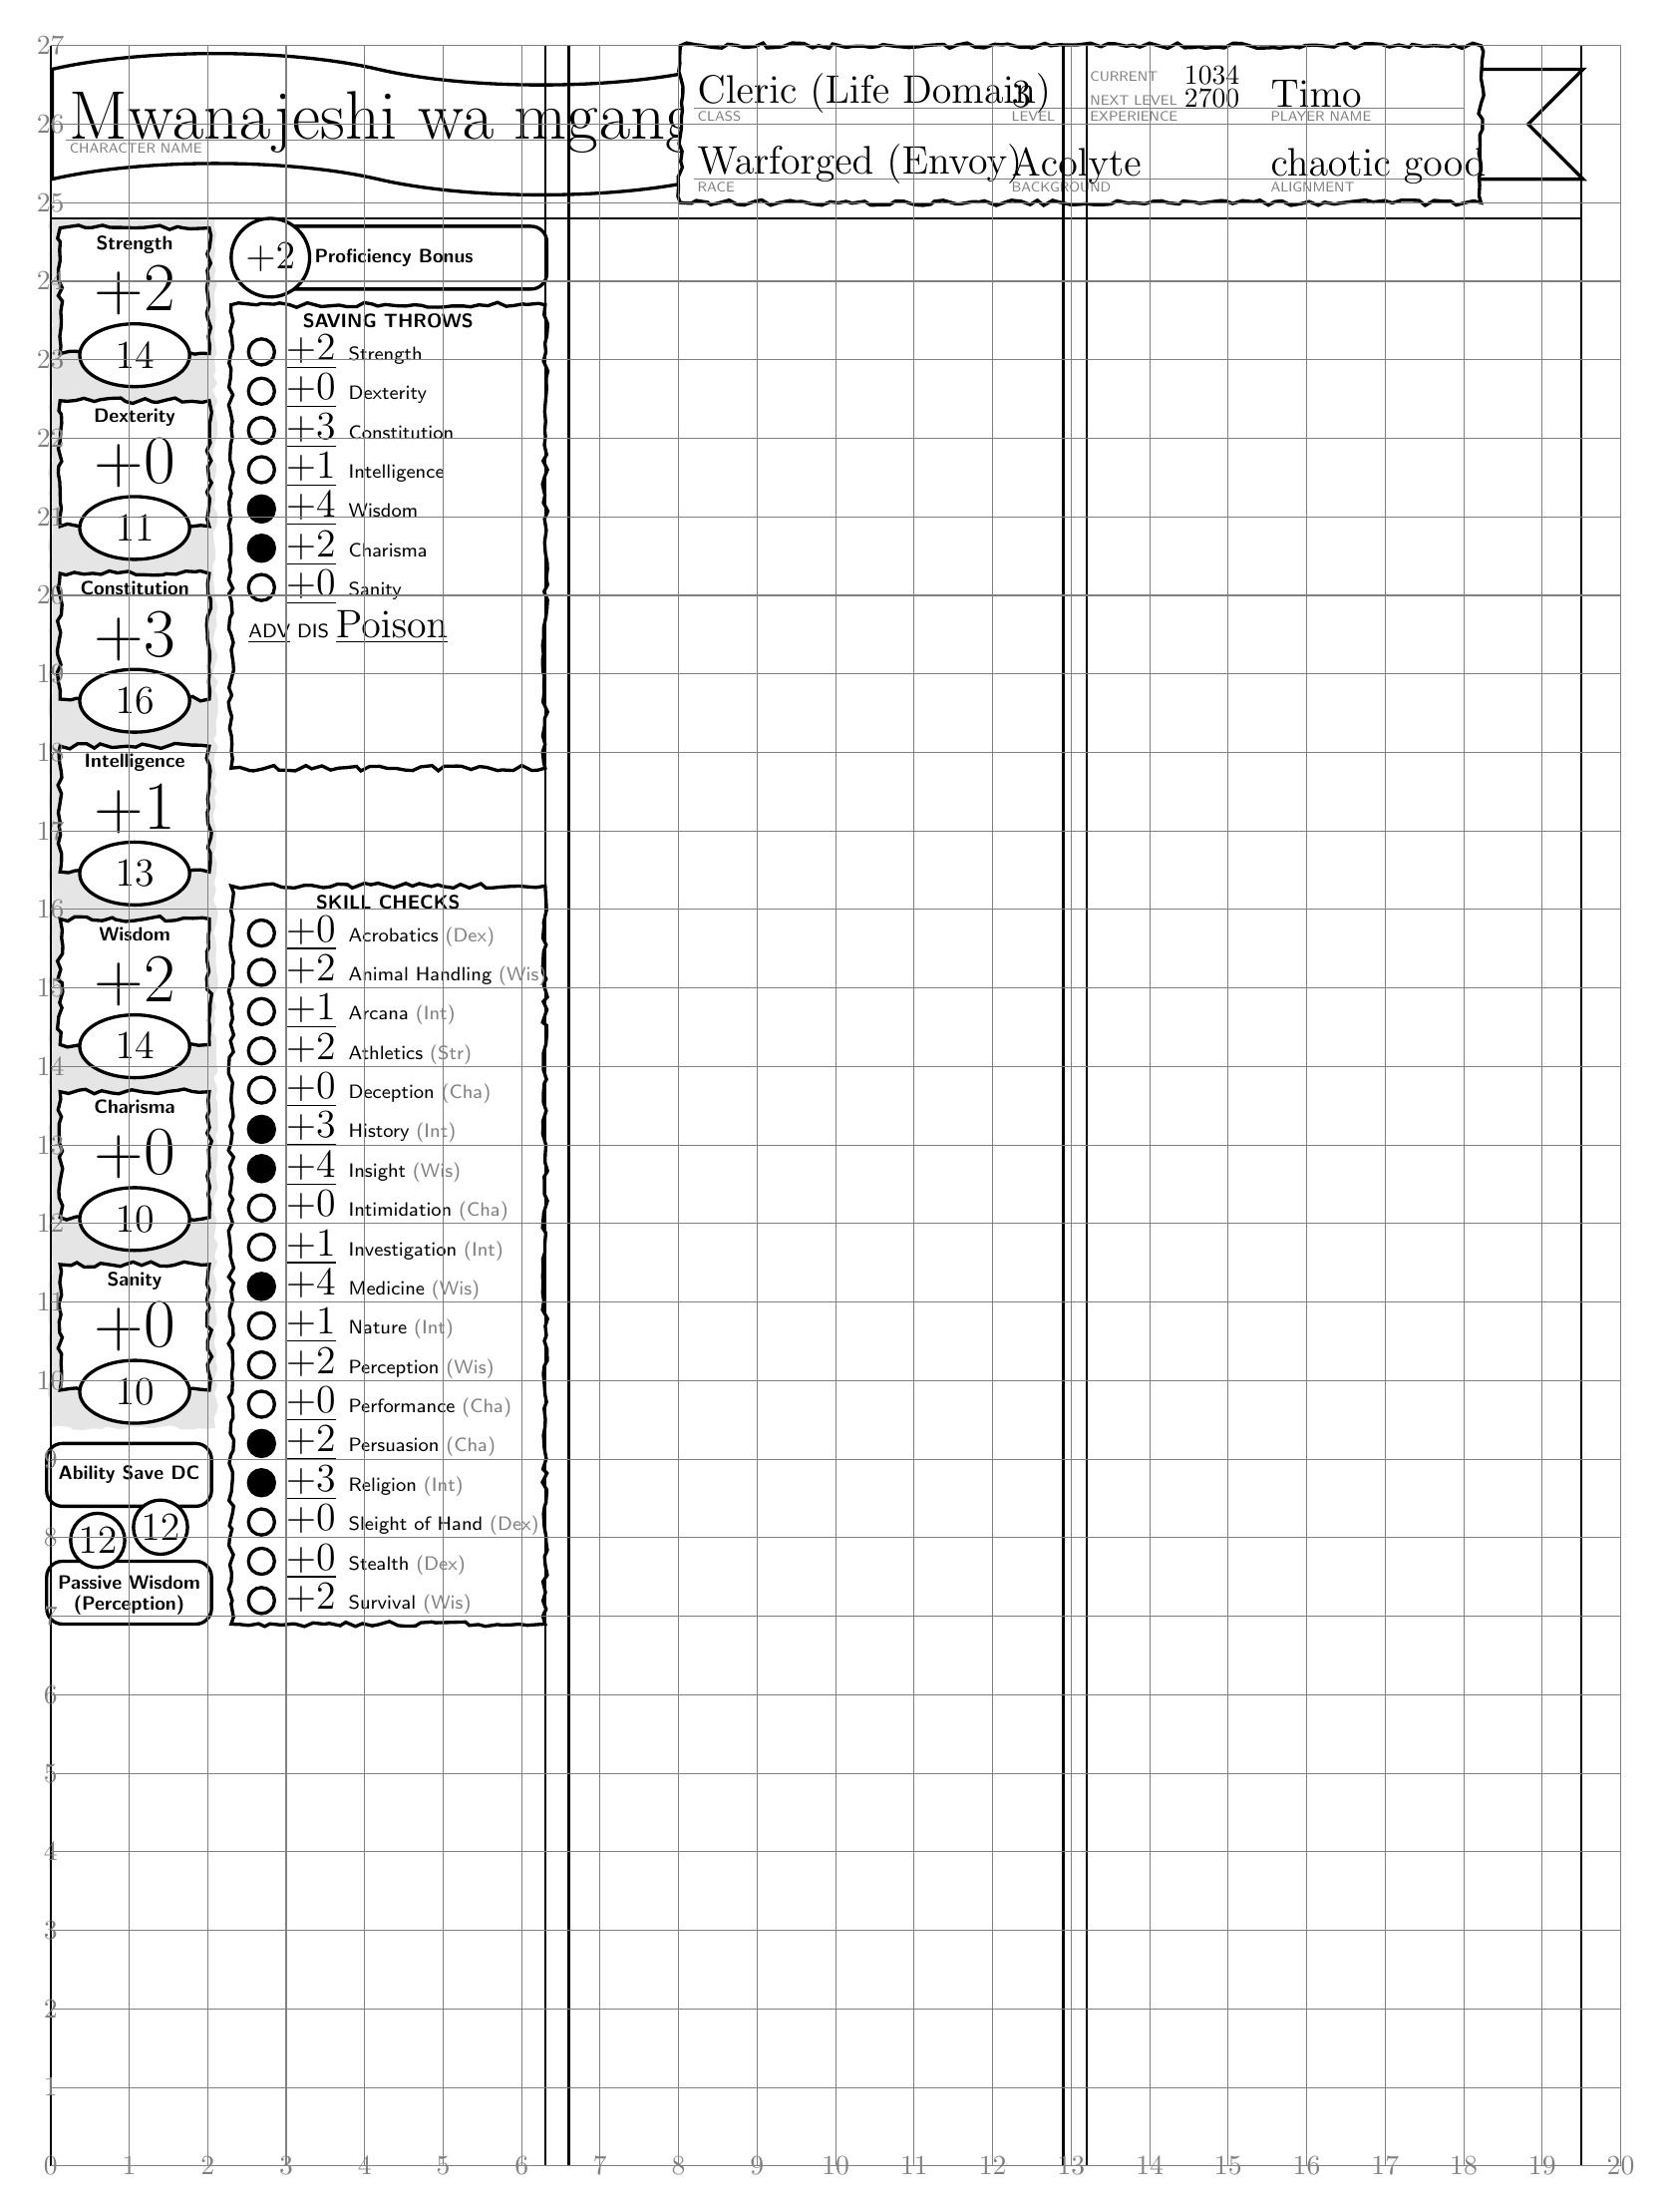
\begin{tikzpicture}
    
    % name box
        % background
        \draw (0,26) node[anchor=west,name box, minimum height=18mm, minimum width=83mm, inner sep=5pt] {};
        % line
        \draw[gray] (0.2,25.8) -- (18.3, 25.8);
        %text
        \draw (0.2,25.8) node[anchor=north west, inner sep=1pt, gray] {\tiny \sffamily CHARACTER NAME} 
                +(0,-0.2) node[anchor=south west, inner sep=1pt, font=\vphantom{Ag}] {\Huge \vName};

% right flag
        % background
        \draw (17,26) node[anchor=west,level box, minimum height=14mm, minimum width=25mm] {};

% big box
        \draw (8,26) node[anchor=west, border box, minimum height=20mm, minimum width=102mm] {};

% upper line
        \draw[gray] (8.2,26.2) -- (18,26.2);

        % class
        \draw (8.2,26.2) node[anchor=north west, inner sep=1pt, gray] {\tiny \sffamily CLASS} 
               +(0,-0.1) node[anchor=south west, inner sep=1pt, font=\vphantom{Ag}] {\Large \vClass};

        % level
        \draw (12.2,26.2) node[anchor=north west, inner sep=1pt, gray] {\tiny \sffamily LEVEL} 
               +(0,-0.1) node[anchor=south west, inner sep=1pt, font=\vphantom{Ag}] {\Large \vLvl};
        
        % XP
        \draw (13.2,26.2) node[anchor=north west, inner sep=1pt, gray] {\tiny \sffamily  EXPERIENCE} 
                +(0,0)  node[anchor=south west, inner sep=1pt, gray] {\tiny \sffamily NEXT LEVEL} 
                +(1.2,-0.1) node[anchor=south west, inner sep=1pt, font=\vphantom{Ag}] { \vnXP}
                +(0,0.3)        node[anchor=south west, inner sep=1pt, gray] {\tiny \sffamily CURRENT}
                +(1.2,.2) node[anchor=south west, inner sep=1pt, font=\vphantom{Ag}] { \vXP};

        % player name
        \draw (15.5,26.2) node[anchor=north west, inner sep=1pt, gray] {\tiny \sffamily PLAYER NAME} 
                +(0,-0.1) node[anchor=south west, inner sep=1pt, font=\vphantom{Ag}] {\Large \vPlayer};


% lower line
        \draw[gray] (8.2,25.3) -- (18,25.3);

        % race
        \draw (8.2,25.3) node[anchor=north west, inner sep=1pt, gray] {\tiny \sffamily RACE} 
               +(0,-0.1) node[anchor=south west, inner sep=1pt, font=\vphantom{Ag}] {\Large \vRace};

        % background
        \draw (12.2,25.3) node[anchor=north west, inner sep=1pt, gray] {\tiny \sffamily BACKGROUND} 
                +(0,-0.1) node[anchor=south west, inner sep=1pt, font=\vphantom{Ag}] {\Large \vBackground};

        % alignment
        \draw (15.5,25.3) node[anchor=north west, inner sep=1pt, gray] {\tiny \sffamily ALIGNMENT} 
                +(0,-0.1) node[anchor=south west, inner sep=1pt, font=\vphantom{Ag}] {\Large \vAlignment};
    % base stats
    \draw[shade box] (0.0,24.8) rectangle  (2.1,9.4);
    % strength
    \draw (0.1,24.7) node[border box, minimum width = 19mm, minimum height = 16mm, anchor=north west] (strength) {\Huge \vStrMod}
        (strength.north) node[anchor=north] {\scriptsize \sffamily \textbf{Strength}}
        (strength.south) node[circle box, minimum width = 14mm, minimum height = 8mm]{\Large \vStr};

    % dexterity
    \draw (0.1,22.5) node[border box, minimum width = 19mm, minimum height = 16mm, anchor=north west] (dexterity) {\Huge \vDexMod}
        (dexterity.north) node[anchor=north] {\scriptsize \sffamily \textbf{Dexterity}}
        (dexterity.south) node[circle box, minimum width = 14mm, minimum height = 8mm]{\Large \vDex};

    % constitution
    \draw (0.1,20.3) node[border box, minimum width = 19mm, minimum height = 16mm, anchor=north west] (constitution) {\Huge \vConMod}
        (constitution.north) node[anchor=north] {\scriptsize \sffamily \textbf{Constitution}}
        (constitution.south) node[circle box, minimum width = 14mm, minimum height = 8mm]{\Large \vCon};

    % intelligence
    \draw (0.1,18.1) node[border box, minimum width = 19mm, minimum height = 16mm, anchor=north west] (intelligence) {\Huge \vIntMod}
        (intelligence.north) node[anchor=north] {\scriptsize \sffamily \textbf{Intelligence}}
        (intelligence.south) node[circle box, minimum width = 14mm, minimum height = 8mm]{\Large \vInt};

    % wisdom
    \draw (0.1,15.9) node[border box, minimum width = 19mm, minimum height = 16mm, anchor=north west] (wisdom) {\Huge \vWisMod}
        (wisdom.north) node[anchor=north] {\scriptsize \sffamily \textbf{Wisdom}}
        (wisdom.south) node[circle box, minimum width = 14mm, minimum height = 8mm]{\Large \vWis};

    % charisma
    \draw (0.1,13.7) node[border box, minimum width = 19mm, minimum height = 16mm, anchor=north west] (charisma) {\Huge \vChaMod}
        (charisma.north) node[anchor=north] {\scriptsize \sffamily \textbf{Charisma}}
        (charisma.south) node[circle box, minimum width = 14mm, minimum height = 8mm]{\Large \vCha};

    % sanity
    \draw (0.1,11.5) node[border box, minimum width = 19mm, minimum height = 16mm, anchor=north west] (sanity) {\Huge \vSanMod}
        (sanity.north) node[anchor=north] {\scriptsize \sffamily \textbf{Sanity}}
        (sanity.south) node[circle box, minimum width = 14mm, minimum height = 8mm]{\Large \vSan};

% additional stats
    % proficiency bonus
    \draw (2.8,24.3) node[anchor=west, rounded corners = 2mm, draw, very thick, fill=white, minimum height=8mm, minimum width=35mm]{}
        node[circle box, circle, minimum width = 10mm] (prof){}
        (prof.east) node[anchor=west, inner sep=1pt]{\scriptsize \sffamily \textbf{Proficiency Bonus}}
        (prof) node{\Large \vProf};
    
    % ability save dc | passive wisdom (perception)
    \draw (1,8.8) node[rounded corners = 2mm, draw, very thick, fill=white, minimum height=8mm, minimum width=21mm](asdc){}
        node[inner sep=1pt]{\scriptsize \sffamily \textbf{Ability Save DC}}
        +(.4,-.3)node[anchor=north, inner sep=1pt, draw, circle, very thick, fill=white]{\Large \vAbilitySave}
        ++(0,-1.5) node[rounded corners = 2mm, draw, very thick, fill=white, minimum height=8mm, minimum width=21mm]{}
        node[anchor=north, inner sep=1pt]{\scriptsize \sffamily \textbf{(Perception)}}
        node[anchor=south, inner sep=1pt]{\scriptsize \sffamily \textbf{Passive Wisdom}}
        +(-.4,.3)node[anchor=south, inner sep=1pt, draw, circle, very thick, fill=white]{\Large \vPerception};
    
% saving throws
    % box
    \draw[border box] (2.3,23.7) rectangle (6.3, 17.8);
    % title
    \draw (4.3,23.7) node[anchor=north] {\scriptsize \sffamily \textbf{SAVING THROWS}};
    
    % strength
    \draw (2.5,23.1) node[anchor=west, draw, very thick, circle, fill=\vStrSaveC, minimum width=1mm] (circ) {}
        (circ.east) node[anchor=west]{\Large \underline{\vStrSave{}} \scriptsize \sffamily Strength};
    % dexterity
    \draw (2.5,22.6) node[anchor=west, draw, very thick, circle, fill=\vDexSaveC, minimum width=1mm] (circ) {}
        (circ.east) node[anchor=west]{\Large \underline{\vDexSave{}} \scriptsize \sffamily Dexterity};
    % constitution
    \draw (2.5,22.1) node[anchor=west, draw, very thick, circle, fill=\vConSaveC, minimum width=1mm] (circ) {}
        (circ.east) node[anchor=west]{\Large \underline{\vConSave{}} \scriptsize \sffamily Constitution};
    % intelligence
    \draw (2.5,21.6) node[anchor=west, draw, very thick, circle, fill=\vIntSaveC, minimum width=1mm] (circ) {}
        (circ.east) node[anchor=west]{\Large \underline{\vIntSave{}} \scriptsize \sffamily Intelligence};
    % wisdom
    \draw (2.5,21.1) node[anchor=west, draw, very thick, circle, fill=\vWisSaveC, minimum width=1mm] (circ) {}
        (circ.east) node[anchor=west]{\Large \underline{\vWisSave{}} \scriptsize \sffamily Wisdom};
    % charisma
    \draw (2.5,20.6) node[anchor=west, draw, very thick, circle, fill=\vChaSaveC, minimum width=1mm] (circ) {}
        (circ.east) node[anchor=west]{\Large \underline{\vChaSave{}} \scriptsize \sffamily Charisma};
    % sanity
    \draw (2.5,20.1) node[anchor=west, draw, very thick, circle, fill=\vSanSaveC, minimum width=1mm] (circ) {}
        (circ.east) node[anchor=west]{\Large \underline{\vSanSave{}} \scriptsize \sffamily Sanity};
    % advantage/disadvantage
    \draw (2.4,19.6) node[anchor=west]{\scriptsize \sffamily \underline{ADV} DIS \rmfamily\Large\underline{Poison}};
    
% skill checks
    % box
    \draw[border box] (2.3, 16.3) rectangle (6.3, 6.9);
    % title
    \draw (4.3,16.3) node[anchor=north] {\scriptsize \sffamily \textbf{SKILL CHECKS}};
    
    % acrobatics
    \draw (2.5,15.7) node[anchor=west, draw, very thick, circle, fill=\vAcroC, minimum width=1mm] (circ) {}
        (circ.east) node[anchor=west]{\Large \underline{\vAcro{}} \scriptsize \sffamily Acrobatics \color{gray}(Dex)};
    % animal handling
    \draw (2.5,15.2) node[anchor=west, draw, very thick, circle, fill=\vAnimC, minimum width=1mm] (circ) {}
        (circ.east) node[anchor=west]{\Large \underline{\vAnim{}} \scriptsize \sffamily Animal Handling \color{gray}(Wis)};
    % arcana
    \draw (2.5,14.7) node[anchor=west, draw, very thick, circle, fill=\vArcaC, minimum width=1mm] (circ) {}
        (circ.east) node[anchor=west]{\Large \underline{\vArca{}} \scriptsize \sffamily Arcana \color{gray}(Int)};
    % athletics
    \draw (2.5,14.2) node[anchor=west, draw, very thick, circle, fill=\vAthlC, minimum width=1mm] (circ) {}
        (circ.east) node[anchor=west]{\Large \underline{\vAthl{}} \scriptsize \sffamily Athletics \color{gray}(Str)};
    % deception
    \draw (2.5,13.7) node[anchor=west, draw, very thick, circle, fill=\vDeceC, minimum width=1mm] (circ) {}
        (circ.east) node[anchor=west]{\Large \underline{\vDece{}} \scriptsize \sffamily Deception \color{gray}(Cha)};
    % history
    \draw (2.5,13.2) node[anchor=west, draw, very thick, circle, fill=\vHistC, minimum width=1mm] (circ) {}
        (circ.east) node[anchor=west]{\Large \underline{\vHist{}} \scriptsize \sffamily History \color{gray}(Int)};
    % insight
    \draw (2.5,12.7) node[anchor=west, draw, very thick, circle, fill=\vInsiC, minimum width=1mm] (circ) {}
        (circ.east) node[anchor=west]{\Large \underline{\vInsi{}} \scriptsize \sffamily Insight \color{gray}(Wis)};
    % intimidation
    \draw (2.5,12.2) node[anchor=west, draw, very thick, circle, fill=\vIntiC, minimum width=1mm] (circ) {}
        (circ.east) node[anchor=west]{\Large \underline{\vInti{}} \scriptsize \sffamily Intimidation \color{gray}(Cha)};
    % investigation
    \draw (2.5,11.7) node[anchor=west, draw, very thick, circle, fill=\vInveC, minimum width=1mm] (circ) {}
        (circ.east) node[anchor=west]{\Large \underline{\vInve{}} \scriptsize \sffamily Investigation \color{gray}(Int)};
    % medicine
    \draw (2.5,11.2) node[anchor=west, draw, very thick, circle, fill=\vMediC, minimum width=1mm] (circ) {}
        (circ.east) node[anchor=west]{\Large \underline{\vMedi{}} \scriptsize \sffamily Medicine \color{gray}(Wis)};
    % nature
    \draw (2.5,10.7) node[anchor=west, draw, very thick, circle, fill=\vNatuC, minimum width=1mm] (circ) {}
        (circ.east) node[anchor=west]{\Large \underline{\vNatu{}} \scriptsize \sffamily Nature \color{gray}(Int)};
    % perception
    \draw (2.5,10.2) node[anchor=west, draw, very thick, circle, fill=\vPercC, minimum width=1mm] (circ) {}
        (circ.east) node[anchor=west]{\Large \underline{\vPerc{}} \scriptsize \sffamily Perception \color{gray}(Wis)};
    % performance
    \draw (2.5,9.7) node[anchor=west, draw, very thick, circle, fill=\vPerfC, minimum width=1mm] (circ) {}
        (circ.east) node[anchor=west]{\Large \underline{\vPerf{}} \scriptsize \sffamily Performance \color{gray}(Cha)};
    % persuasion
    \draw (2.5,9.2) node[anchor=west, draw, very thick, circle, fill=\vPersC, minimum width=1mm] (circ) {}
        (circ.east) node[anchor=west]{\Large \underline{\vPers{}} \scriptsize \sffamily Persuasion \color{gray}(Cha)};
    % religion
    \draw (2.5,8.7) node[anchor=west, draw, very thick, circle, fill=\vReliC, minimum width=1mm] (circ) {}
        (circ.east) node[anchor=west]{\Large \underline{\vReli{}} \scriptsize \sffamily Religion \color{gray}(Int)};
    % sleight of hand
    \draw (2.5,8.2) node[anchor=west, draw, very thick, circle, fill=\vSleiC, minimum width=1mm] (circ) {}
        (circ.east) node[anchor=west]{\Large \underline{\vSlei{}} \scriptsize \sffamily Sleight of Hand \color{gray}(Dex)};
    % stealth
    \draw (2.5,7.7) node[anchor=west, draw, very thick, circle, fill=\vSteaC, minimum width=1mm] (circ) {}
        (circ.east) node[anchor=west]{\Large \underline{\vStea{}} \scriptsize \sffamily Stealth \color{gray}(Dex)};
    % survival
    \draw (2.5,7.2) node[anchor=west, draw, very thick, circle, fill=\vSurvC, minimum width=1mm] (circ) {}
        (circ.east) node[anchor=west]{\Large \underline{\vSurv{}} \scriptsize \sffamily Survival \color{gray}(Wis)};

    

    %% column width is 6.3 cm with 3 mm spacing
\draw[thick]    
    % vertical lines from left to right
    (0, 0) -- +(0, 27)
    (6.3, 0) -- +(0, 27)
    (6.6, 0) -- +(0, 27)
    (12.9, 0) -- +(0, 27)
    (13.2, 0) -- +(0, 27)
    (19.5, 0) -- +(0, 27)
    % horizontal line
    (0,24.8) -- +(19.5, 0);
    \draw[gray] (0,0) node{0} -- (20,0)
    (0,1)  node{1} -- (20,1)
    (0,2)  node{2} -- (20,2)
    (0,3)  node{3} -- (20,3)
    (0,4)  node{4} -- (20,4)
    (0,5)  node{5} -- (20,5)
    (0,6)  node{6} -- (20,6)
    (0,7)  node{7} -- (20,7)
    (0,8)  node{8} -- (20,8)
    (0,9)  node{9} -- (20,9)
    (0,10) node{10} -- (20,10)
    (0,11) node{11} -- (20,11)
    (0,12) node{12} -- (20,12)
    (0,13) node{13} -- (20,13)
    (0,14) node{14} -- (20,14)
    (0,15) node{15} -- (20,15)
    (0,16) node{16} -- (20,16)
    (0,17) node{17} -- (20,17)
    (0,18) node{18} -- (20,18)
    (0,19) node{19} -- (20,19)
    (0,20) node{20} -- (20,20)
    (0,21) node{21} -- (20,21)
    (0,22) node{22} -- (20,22)
    (0,23) node{23} -- (20,23)
    (0,24) node{24} -- (20,24)
    (0,25) node{25} -- (20,25)
    (0,26) node{26} -- (20,26)
    (0,27) node{27} -- (20,27)
    (1,0)  node{1} -- (1,27)
    (2,0)  node{2} -- (2,27)
    (3,0)  node{3} -- (3,27)
    (4,0)  node{4} -- (4,27)
    (5,0)  node{5} -- (5,27)
    (6,0)  node{6} -- (6,27)
    (7,0)  node{7} -- (7,27)
    (8,0)  node{8} -- (8,27)
    (9,0)  node{9} -- (9,27)
    (10,0) node{10} -- (10,27)
    (11,0) node{11} -- (11,27)
    (12,0) node{12} -- (12,27)
    (13,0) node{13} -- (13,27)
    (14,0) node{14} -- (14,27)
    (15,0) node{15} -- (15,27)
    (16,0) node{16} -- (16,27)
    (17,0) node{17} -- (17,27)
    (18,0) node{18} -- (18,27)
    (19,0) node{19} -- (19,27)
    (20,0) node{20} -- (20,27);
    
\end{tikzpicture}

\end{document}
